\documentclass{article}

\usepackage{graphicx, caption, subcaption, amsmath}

\usepackage{hyperref}
\hypersetup{
    colorlinks,
    citecolor=black,
    linkcolor=black,
    urlcolor=blue
}

% Automatic float-barrier around subsections
\usepackage[section]{placeins}
\makeatletter
\AtBeginDocument{%
  \expandafter\renewcommand\expandafter\subsection\expandafter{%
    \expandafter\@fb@secFB\subsection
  }%
}
\makeatother

\begin{document}

\title{A Gentle Introduction to Elliptic Curve Cryptography}
\author{Tanner Prynn}
\maketitle

\tableofcontents
\clearpage

\section*{Foreword}
\addcontentsline{toc}{section}{Foreword}

\section{Elliptic Curves}

\subsection{What is an Elliptic Curve?}
An \textbf{elliptic curve} is a set of points satisfying an equation of the form
$$y^2 = x^3 + ax + b$$
for coefficients $a,b$ and variables $x,y$ in some field $F$ (of characteristic not 2 or 3). 
We place one additional restriction on an elliptic curve, which is that
$4a^3 + 27b^2 \neq 0$.
This condition ensures that the curve is \textit{non-singular}, which allows us to find a tangent line to any point on the curve \cite[$\S$3.1]{ecc-guide}.

Let's start with a few examples of curves, plotted over the real numbers.
Figure \ref{fig:ec-plot} shows a simple elliptic curve.
It has three real roots, which correspond to the zeroes of the polynomial $x^3 - 3x + 1$.
Figure \ref{fig:ec-plot2} shows the elliptic curve $y^2 = x^3 - 2x + 2$, which only has one real root.

\begin{figure}[h]
\centering
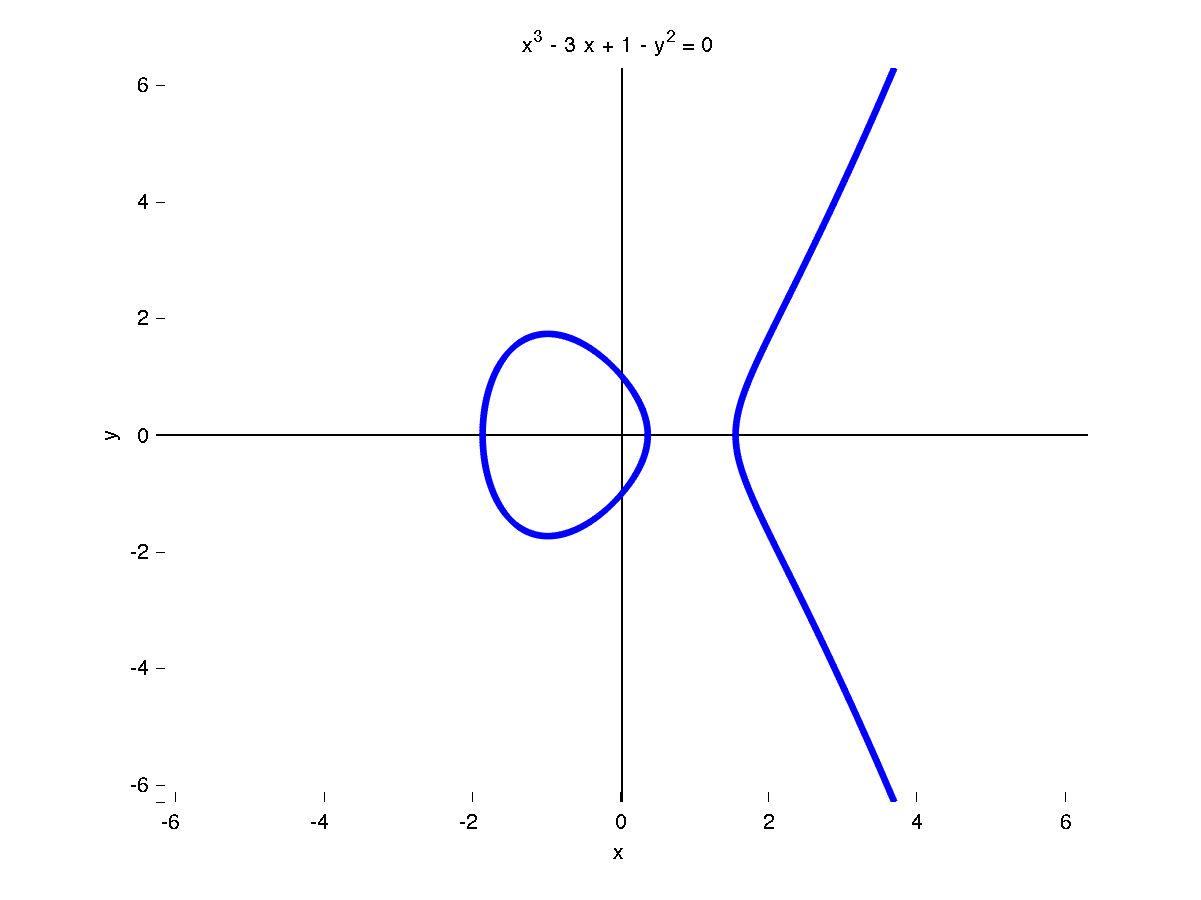
\includegraphics[width=\textwidth]{images/ec1.png}
\caption{The elliptic curve $y^2 = x^3 - 3x + 1$}
\label{fig:ec-plot}
\end{figure}

\begin{figure}[h]
\centering
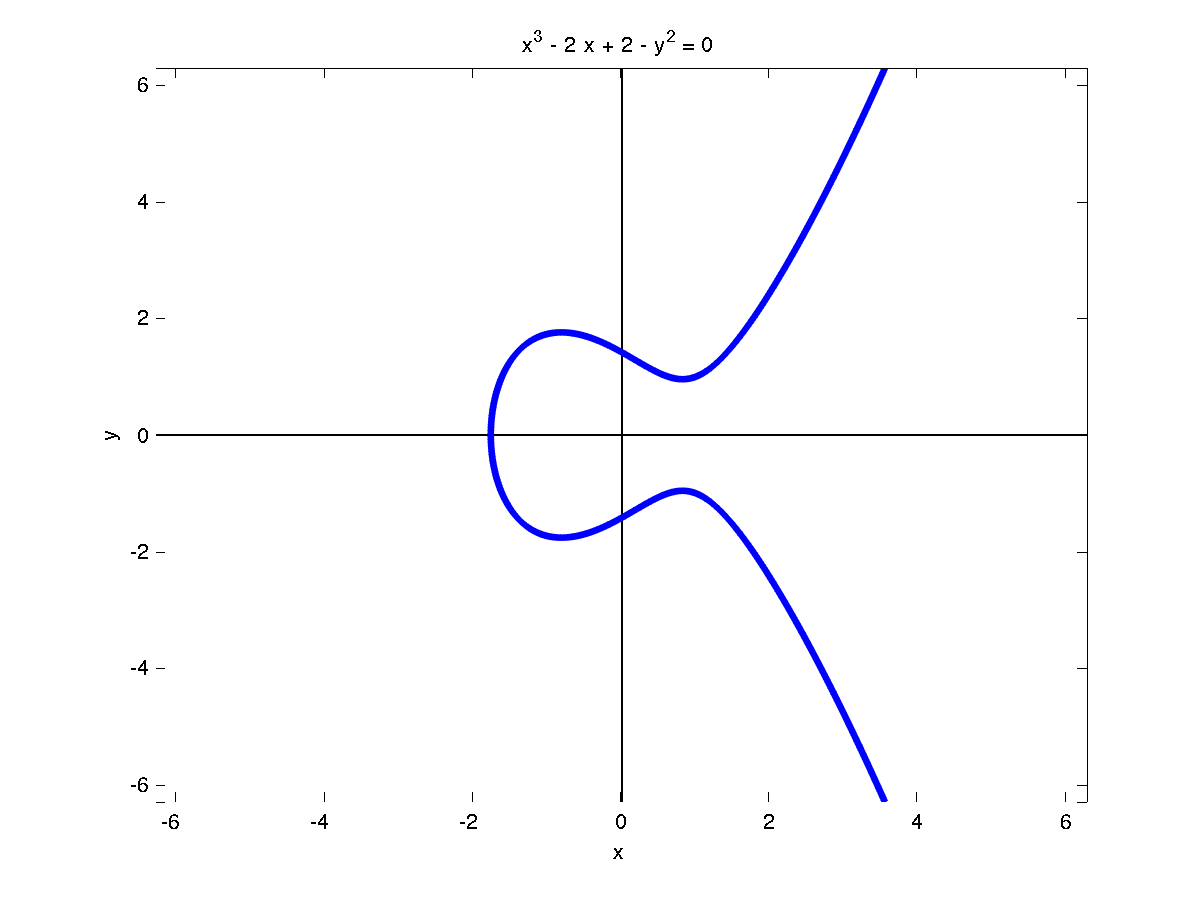
\includegraphics[width=\textwidth]{images/ec4g.png}
\caption{The elliptic curve $y^2 = x^3 - 2x + 2$}
\label{fig:ec-plot2}
\end{figure}

Figure \ref{fig:ec-singular} shows two singular curves.
To define a group operation on the points of the curve, we need to be able to take a tangent line to each point.
So we avoid these cases with that additional restriction on the coefficients.

\begin{figure}[h]
\centering

\begin{subfigure}{.5\textwidth}
	\centering
	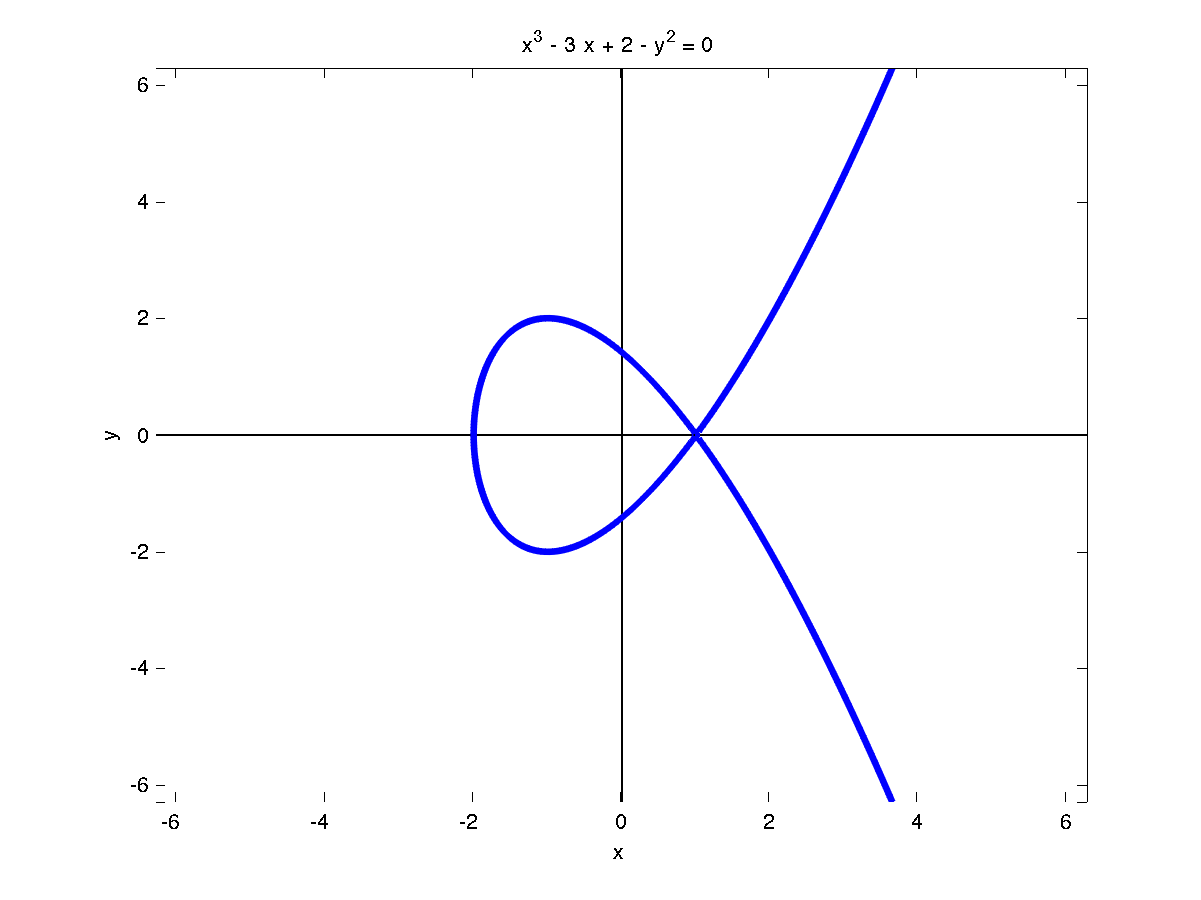
\includegraphics[width=1\linewidth]{images/ec2.png}
	\caption{The curve $y^2 = x^3 - 3x + 2$}
\end{subfigure}%
~%
\begin{subfigure}{.5\textwidth}
	\centering
	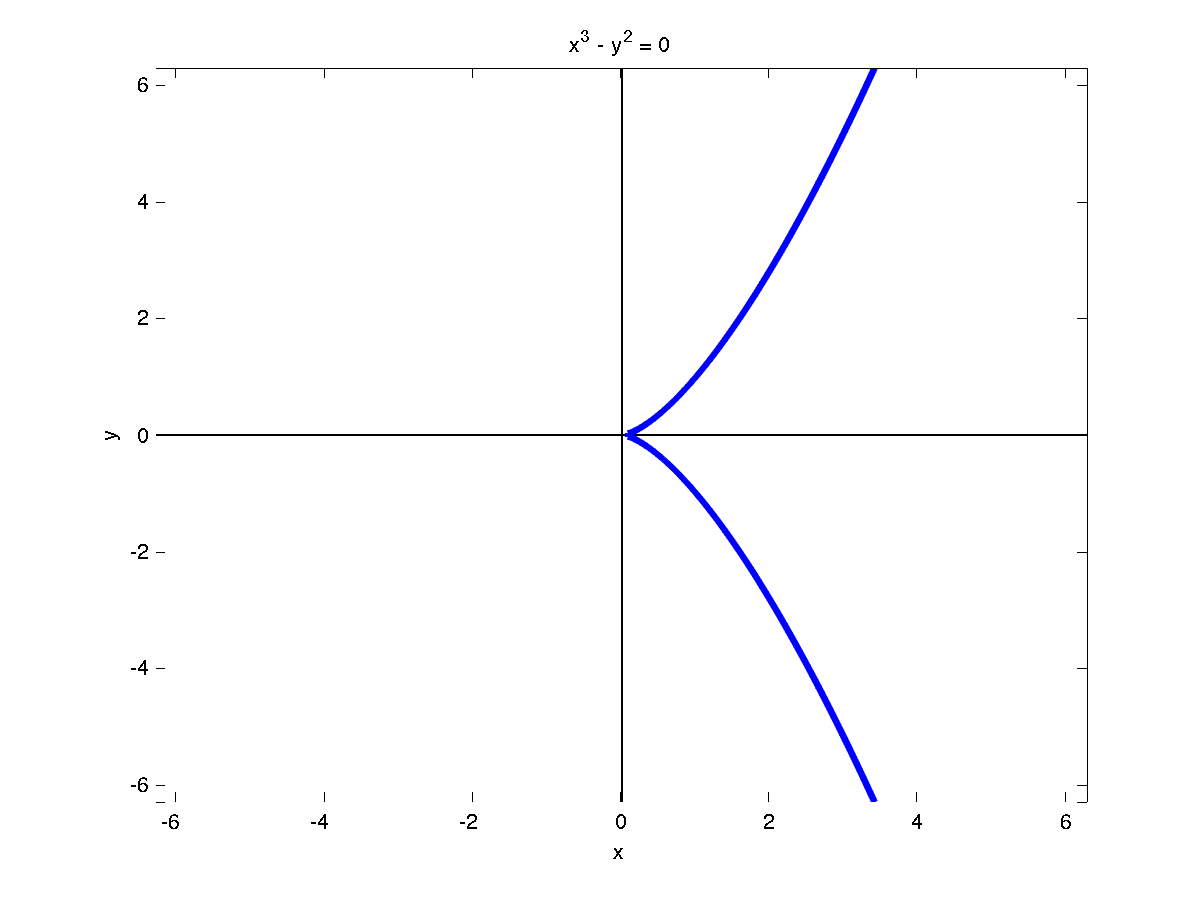
\includegraphics[width=1\linewidth]{images/ec3.png}
	\caption{The curve $y^2 = x^3$}
\end{subfigure}

\caption{These curves have a `singularity': a point where the tangent is not clearly defined.}
\label{fig:ec-singular}
\end{figure}

\subsection{Defining a Group Operation}
Now, we have an equation for a curve, and we can define the set of points 
$$C = \{(x,y) \mid x,y \in F \text{ and } y^2 = x^3 + ax + b\}$$
which is a subset of of the plane $F^2$.
We want to make the set $C$ into a group, so we need to define an operation on it.
Let's call that operation $*$, and we'll define $P_1 * P_2$ as the third intersection of the line through $P_1$ and $P_2$ which lies on the curve $C$.
Figure \ref{fig:ec-3rd-intersection} shows this operation for the simple case of two different points.

\begin{figure}[h]
\centering
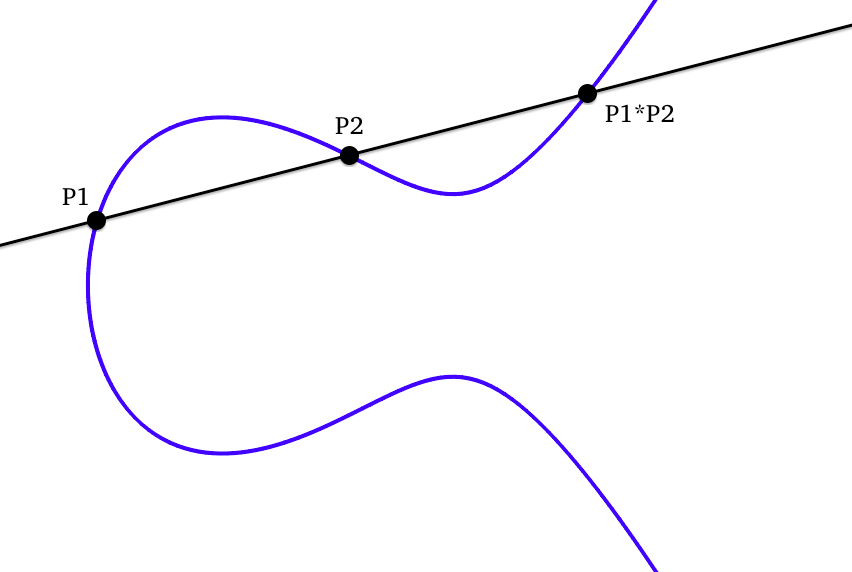
\includegraphics[width=0.6\textwidth]{images/ec4-star.png}
\caption{Finding the third point of intersection on the curve $y^2 = x^3 - 2x + 2$}
\label{fig:ec-3rd-intersection}
\end{figure}

What other cases are there?
First, we need to define $*$ when $P_1 = P_2$.
We want to have the line through $P_1$ hit the curve at exactly two points, $P_1$ and $P_1*P_1$.
To achieve this, let the line through $P_1$ be the tangent to the curve.
Then the tangent line intersects the curve at one additional point, as desired (figure \ref{fig:ec-tangent}) \cite[$\S$I.2]{rational-points}.

\begin{figure}[h]
\centering
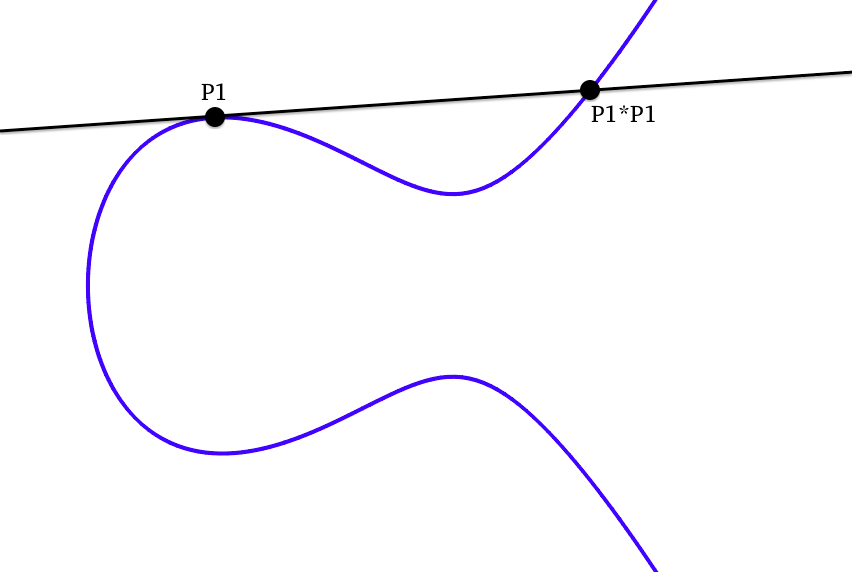
\includegraphics[width=0.6\textwidth]{images/ec4-tangent.png}
\caption{A tangent line intersects the curve at two points.}
\label{fig:ec-tangent}
\end{figure}

Now, we come to the case of a vertical line.
A vertical line will intersect our curve at exactly two points, because the curve is symmetric over the $x$-axis.
But those two points will violate our $*$ operation, because there isn't a third-point where the line intersects the curve (figure \ref{fig:ec-infinity}).
This leads us to take an idea from projective geometry: that there is an extra point on the curve called the \textit{point at infinity}.

\begin{figure}[h]
\centering
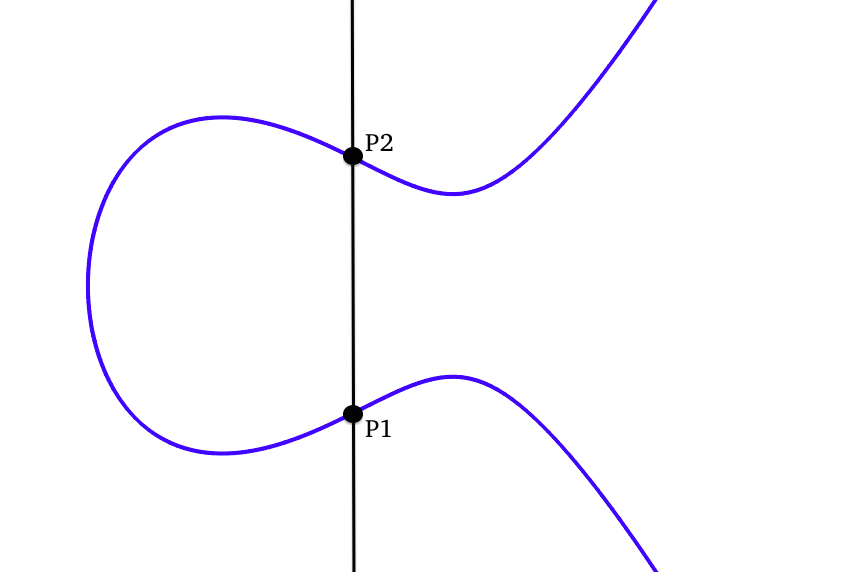
\includegraphics[width=0.6\textwidth]{images/ec4-infinity.png}
\caption{A vertical line only intersects the curve at two points.}
\label{fig:ec-infinity}
\end{figure}

The point at infinity (denoted $\infty$) is a point in the projective plane, so there isn't an intuitive way to draw it in our standard plane.
However, we can understand $\infty$ as `outside' of the plane, and simply treat it as a special geometric object.
As a benefit, we can take the third intersection of a vertical line to be $\infty$.
We then need to redefine the set of points $C$ to include $\infty$:
$$C = \{\infty\} \cup \{(x,y) \mid x,y \in F \text{ and } y^2 = x^3 + ax + b\}$$
Thus we have disposed of this problematic case \cite[$\S$2.2]{washington}.

Having $\infty$ on our curve is also useful because it is a unique point which exists on every elliptic curve.
This makes it an ideal candidate for the identity element of our group operation.
We need to redefine our operation to make this true, however.
If we reconsider the case of the vertical line, we have two points $P_1$ and $P_2$ such that $P_1 * P_2 = \infty$.
Because the curve is symmetric, all we need to do to get $P_1$ from $P_2$ is to reflect over the $x$-axis.

Let's define a new operation $+$ and say that, for any point $P \in C$, $P = P+\infty = \infty+P$.
To produce $+$ from our previous operation $*$, we only need to add one additional step: a reflection over the $x$-axis.
We will see later that this operation is commutative, which is why we chose to use the addition symbol \cite[$\S$2.2]{washington}.
Figure \ref{fig:ec-plus} revisits the previous cases to show how this new operation works.

\begin{figure}[h]
\centering

\begin{subfigure}{.5\textwidth}
	\centering
	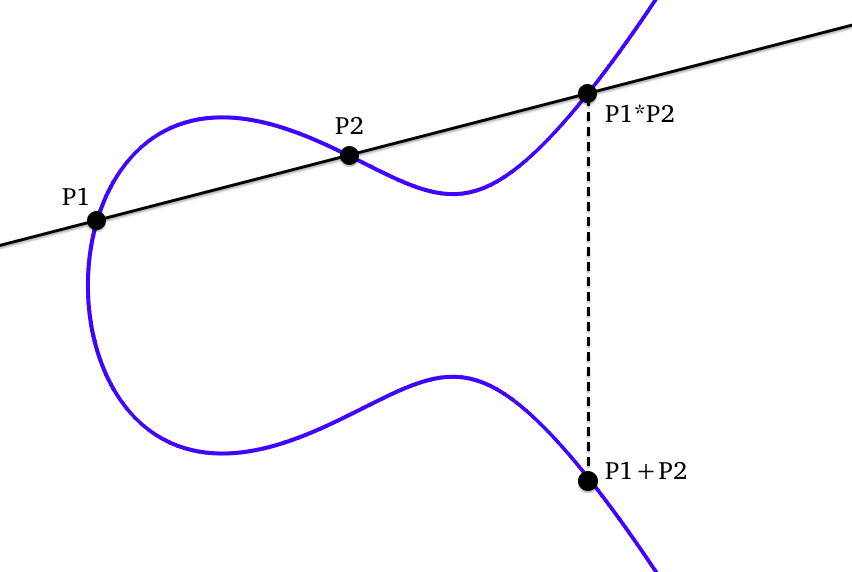
\includegraphics[width=1\linewidth]{images/ec4-plus.png}
	\label{fig:ec-plus-1}
\end{subfigure}%
~%
\begin{subfigure}{.5\textwidth}
	\centering
	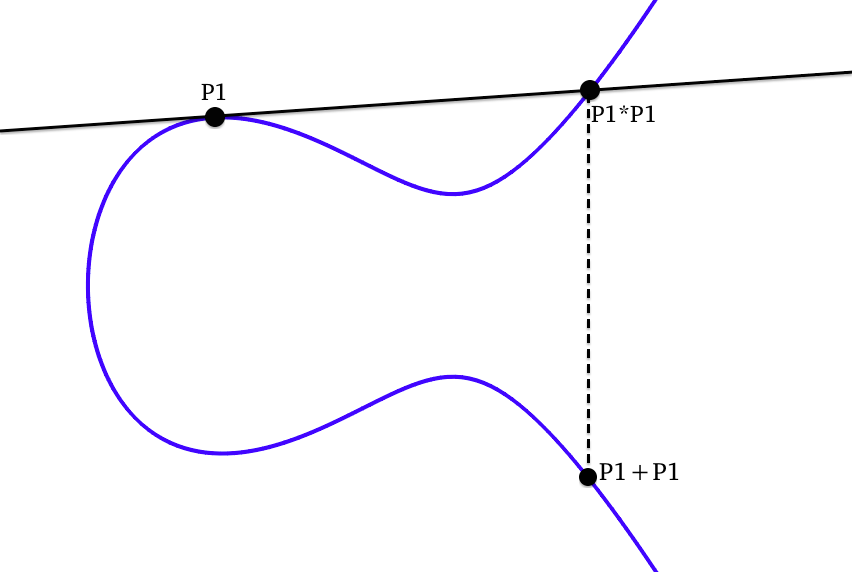
\includegraphics[width=1\linewidth]{images/ec4-plus-tangent.png}
	\label{fig:ec-plus-2}
\end{subfigure}

\caption{The $+$ operation for two points on an elliptic curve}

\label{fig:ec-plus}
\end{figure}

\subsection{Deriving the Group Law}
\textbf{Outline only}

\subsubsection{Addition}
Math

\subsubsection{Doubling}
Math

\subsubsection{Inverses}
-(x,y) = (x,-y)

\subsubsection{Closure}
Follows from above formulas and closure of field F

\subsubsection{Commutativity}
The line through points a,b is the same as the line through points b,a

\subsubsection{Associativity}
Is it worth proving associativity? I think it's not. The proof is quite long and involved. I think simply offering a reference is enough.

\subsection{Weierstrass Form and Acceptable Changes of Variables}
Weierstrass Form is not the `only' form of an elliptic curve. We can use an acceptable changes of variables/biration equivalence to write other forms of elliptic curves.

E.g. Montgomery Curve

\clearpage

\section{The Discrete Logarithm Problem}

\subsection{Trap-Door Functions}

\subsection{Attacks on Discrete Logarithms}

\clearpage

\section{Elliptic-Curve Diffie-Hellman Exchange}

\subsection{The Diffie-Hellman Key Exchange}

\subsection{Implementation Details of ECDH}

\clearpage

\begin{thebibliography}{9}

\bibitem{ecc-guide}
	Darrel Hankerson, Alfred J. Menezes, and Scott Vanstone:
	\emph{Guide to Elliptic Curve Cryptography}.
	Springer,
	2004.

\bibitem{rational-points}
	Joseph Silverman and John Tate:
	\emph{Rational Points on Elliptic Curves}.
	Springer,
	1994.

\bibitem{washington}
	Lawrence Washington:
	\emph{Elliptic Curves: Number Theory and Cryptography}.
	Chapman and Hall/CRC,
	2nd edition,
	2008.

\end{thebibliography}

\end{document}